\documentclass[11pt,english]{article}
\usepackage[T1]{fontenc}
\usepackage{babel}
\usepackage[margin=1in]{geometry}
\usepackage{graphicx}
\usepackage{amsmath, amsfonts, amsthm, amssymb}
\usepackage{color}
\usepackage{enumerate}

% \hrule with 0.3cm spaces above and below
\newcommand{\myhrule}{\vspace{0.3cm}\hrule\vspace{0.3cm}}
% skip page-numbering on the Title Page
\pagenumbering{gobble}

%%%%%%%%%%%%%%%%%%%%%%%%HEADER%%%%%%%%%%%%%%%%%%%%%%%%%%%%%
\title{How to Download, Install, and Configure Python 2.7\\
on 64-bit Windows 7}
\author{
  Shashank Singh\\
  \texttt{sss1@andrew.cmu.edu}
  \and
  Jimmy Zong\\
  \texttt{yzong@cmu.edu}
}
%%%%%%%%%%%%%%%%%%%%%%%%%%%%%%%%%%%%%%%%%%%%%%%%%%%%%%%%%%%

\begin{document}
% TITLE PAGE
\begin{titlepage}
\maketitle
\vfill
{\bf \color{red} \underline{Important:}} Before installing Python 2.7, you must
uninstall any other versions of Python. Failure to do so may result in
incompatibility issues. See \texttt{http://www.wikihow.com/Uninstall-Python}
for instructions on how to uninstall Python.
\myhrule
{\bf Target Audience:}\\
Anyone who knows what Python 2.7 is and wants their computer to be able to run
Python 2.7 scripts. We assume some familiarity with web browsing, including
downloading and opening files.
\myhrule
{\bf Objective:} This document explains how to download, install, and
configure Python for your 64-bit Windows 7 computer, allowing all users of your
computer to run Python scripts and programs from the Windows Command Line.
\myhrule
{\bf You will need:}\\
A 64-bit computer with Windows 7 and an internet connection. You must also have
administrative priveleges on this computer.
\myhrule
{\bf Duration:}\\
Completing these {\bf 5 steps} should take about {\bf 10 minutes}.
\myhrule
{\bf Outcome:}\\
After completing these steps, all users on your computer should be able to run
the Python 2.7 Interpreter, as well as Python 2.7 scripts ({\bf .py} files) and
compiled Python 2.7 programs ({\bf .pyc} files).\\\\
This document does not explain how to use Python 2.7; for instructions on how
to use Python 2.7, see \texttt{http://www.python.org/}.
\vspace{2cm}

{\bf Step 1} (on page 1) will show you how to download the Python
installer.
\myhrule
\end{titlepage}

\pagenumbering{arabic}
% STEP 1
{\Large {\bf Step 1: Downloading the Python Installer}}
\myhrule
{\bf In this step, you will download the Python Installer, a program which will
install Python on your computer. This step has 2 substeps.}
\begin{enumerate}[a.]
\item Open the URL \texttt{http://www.python.org/download/releases/2.7.5/} in
your web browser.
\item Locate and single-click ``Windows X86-64 MSI Installer'' (highlighted in
Figure \ref{fig:dia1}) to download the installer.
\end{enumerate}
\begin{figure}[h]
\begin{center}
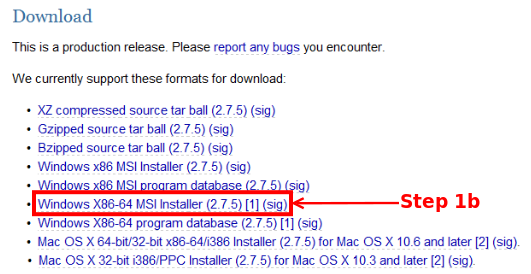
\includegraphics[width=0.6\textwidth]{dia1}
\end{center}
\caption{Link to Python Installer (step 1b.)}
\label{fig:dia1}
\end{figure}
\vfill
{\bf Step 2} (on page 2) will show you how to use this file to Install Python.
\myhrule

% STEP 2
\newpage
{\Large {\bf Step 2: Installing Python}}
\myhrule
{\bf This step has 6 substeps.}
\begin{enumerate}[a.]
\item Locate the file \texttt{python-2.7.5.msi} on your computer. The file
location will depend on your web-browser's download settings.
\item Double-click \texttt{python-2.7.5.msi} to run it.
\item If a `Security Warning' window appears, click ``Run'' (labeled in Figure
\ref{fig:dia2}).
\begin{figure}[h]
\begin{center}
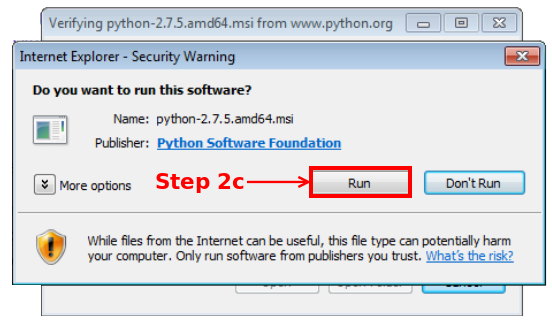
\includegraphics[width=0.5\textwidth]{dia2}
\end{center}
\vspace{-0.5cm}
\caption{``Security Warning'' window (step 2b.)}
\label{fig:dia2}
\end{figure}
\item In the next window, click ``Next'' without changing any settings.
\item Typically, the default installation directory will suffice. To change the
installation directory, select from the drop down menu or type the directory
path in the text box labeled in Figure \ref{fig:dia3}. {\bf Choose
a directory that is currently empty, or there is a chance that your
files will be overwritten. Also, it is IMPORTANT that you remember the
installation directory you choose, because you will need this for Step 4.}
Click ``Next'' when done.
\begin{figure}[h]
\begin{center}
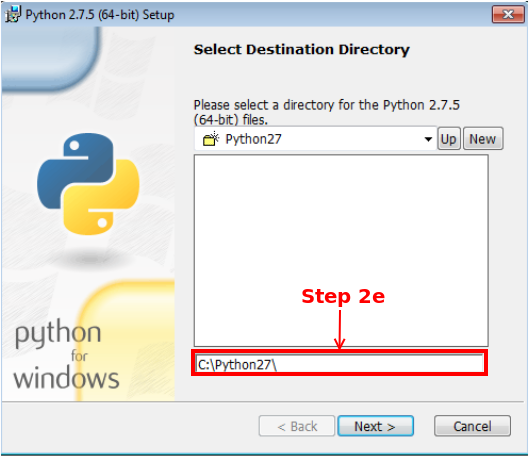
\includegraphics[width=0.48\textwidth]{dia3}
\end{center}
\vspace{-0.5cm}
\caption{Choosing an Installation Directory window (step 2e.)}
\label{fig:dia3}
\end{figure}
\newpage
\item Click ``Next'' without changing any settings. Wait for the installation
to complete. If, during the installation, a ``User Account Control'' window
appears, click  ``Yes'' (labeled in Figure \ref{fig:dia11}). Once the
installation is complete, click ``Finish'' to close the installation program.
\end{enumerate}
\begin{figure}[h]
\begin{center}
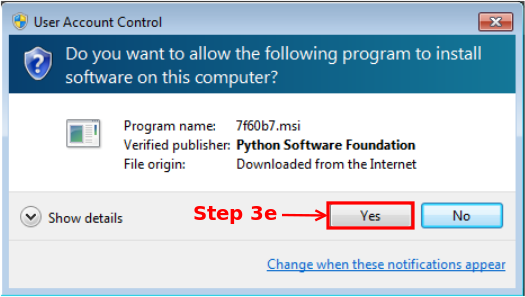
\includegraphics[width=0.55\textwidth]{dia11}
\end{center}
\caption{The User Account Control window (step 2f.)}
\label{fig:dia11}
\end{figure}
\vfill
{\bf Step 3} (on page 4) will begin explaining how to configure your computer
to run Python.
\myhrule

% STEP 3
\newpage
{\Large {\bf Step 3: Opening the Environment Variables Menu}}
\myhrule
{\bf Now, you will modify the Path Environment Variable. This is necessary for
your command line to run Python files. This step has 6 substeps}.
\begin{enumerate}[a.]
\item Open the Start Menu by clicking the bottom left corner of your screen
(labeled in Figure \ref{fig:dia4}).
\item Click on ``Control Panel'' (labeled in Figure \ref{fig:dia4}) to open
the Control Panel.
\begin{figure}[h]
\begin{center}
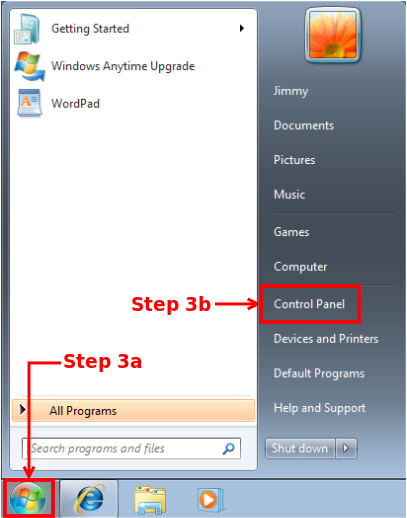
\includegraphics[width=0.35\textwidth]{dia4}
\end{center}
\vspace{-0.5cm}
\caption{The Start Menu (steps 3a. and 3b.)}
\label{fig:dia4}
\end{figure}
\item Type ``advanced'' (without quotes) into the Search Box in the top right
corner of the Control Panel window (as in Figure \ref{fig:dia5}).
\item Click ``View advanced system settings'' (labeled in Figure
\ref{fig:dia5}).
\begin{figure}[h]
\begin{center}
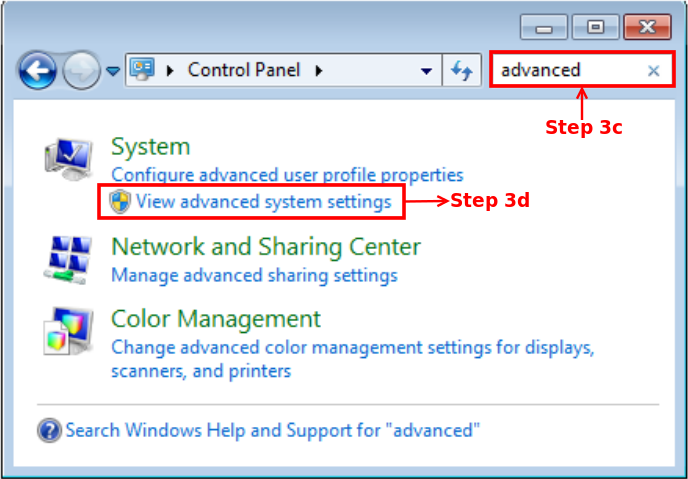
\includegraphics[width=0.6\textwidth]{dia5}
\end{center}
\vspace{-0.5cm}
\caption{The Control Panel (steps 3c. and 3d.)}
\label{fig:dia5}
\end{figure}
\item In the ``System Properties'' window, click ``Environment
Variables'' (labeled in Figure \ref{fig:dia6}).
\begin{figure}[h]
\begin{center}
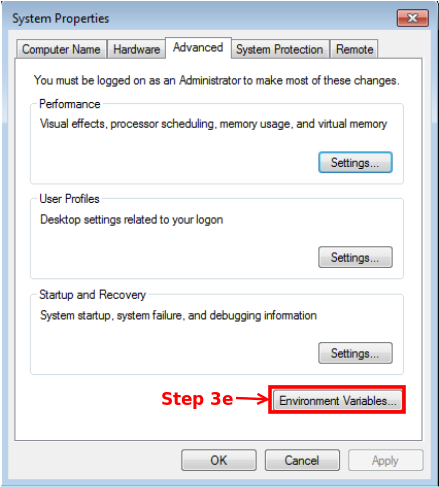
\includegraphics[width=0.5\textwidth]{dia6}
\end{center}
\vspace{-0.5cm}
\caption{System Properties window and the Environment Variables button (step
3f.)}
\label{fig:dia6}
\end{figure}
\end{enumerate}
\vfill
{\bf Step 4} (on page 6) will show you how to modify the Path Environment
Variable.
\myhrule

% STEP 4
\newpage
{\Large {\bf Step 4: Modifying the Path Environment Variable}}
\myhrule
{\bf In this step, you will modify the Path environment variable, telling your
command line the location of your Python Installation. This step has
3 substeps.}\\

{\bf \color{red} \underline{Caution:}} Important system services depend on
Environment Variables. Do not modify any Environment Variables
except Path. Only {\bf add} information to the Path variable. If you make a
mistake, click ``Cancel'' in the bottom right corner of the current window to
undo any changes.

\begin{enumerate}[a.]
\item In the ``Environment Variables'' window that appears, under the ``System
Variables'' section scroll down to locate the Path variable, as shown in Figure
\ref{fig:dia7}. Double-click the word ``Path.''
\begin{figure}[h]
\begin{center}
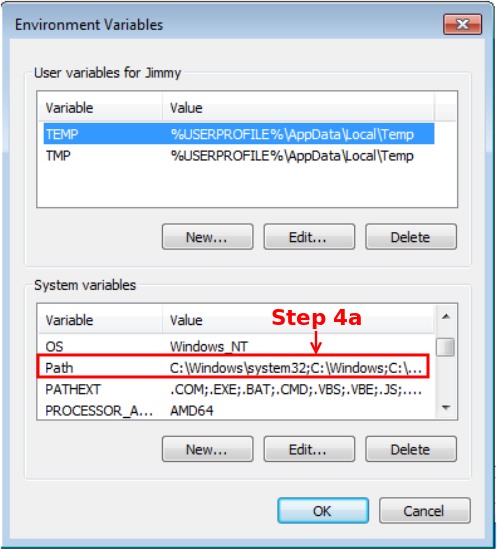
\includegraphics[width=0.4\textwidth]{dia7}
\end{center}
\vspace{-0.5cm}
\caption{Environment Variables window and the Path variable (step 4a.)}
\label{fig:dia7}
\end{figure}
\item An ``Edit System Variable'' window will appear. In the ``Variable value''
box ({\bf do not delete anything!}), at the end of the current value, add
``\texttt{;C:}'' followed by the name of the directory selected in step 2e.
(for the default directory, add ``\texttt{;C:\textbackslash Python27}'' as
shown in Figure \ref{fig:dia8}).
\begin{figure}[h]
\begin{center}
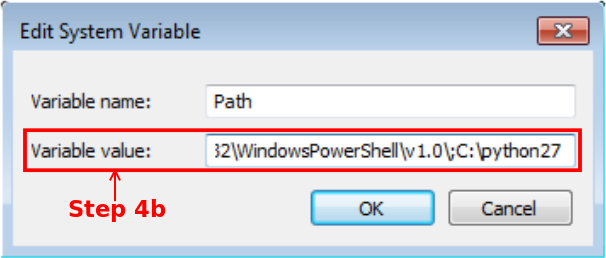
\includegraphics[width=0.4\textwidth]{dia8}
\end{center}
\vspace{-0.5cm}
\caption{The Edit System Variable window (step 4b.)}
\label{fig:dia8}
\end{figure}
\item Click ``OK'' to close each of the ``Edit System Variable'' and
``Environment Variables'' windows.
\end{enumerate}
\vfill
You now have Python 2.7 installed and configured on your computer. {\bf Step 5}
(on page 7) will show you how to access the Python interpreter to start using
Python right away.
\myhrule

% STEP 5
\newpage
{\Large {\bf Step 5: Opening the Python Interpreter}}
\myhrule
{\bf In this step, you will verify that the previous steps worked by opening
the Command Line Python Interpreter. This step has 4 substeps.}\\

\begin{enumerate}[a.]
\item Open the Start Menu by clicking the bottom left corner of your screen
(labeled in Figure \ref{fig:dia9}).
\item In the search box, type ``cmd'' (without quotes), as shown in Figure
\ref{fig:dia9}).
\item Click on ``cmd'' (labeled in Figure \ref{fig:dia9}).
\begin{figure}[h]
\begin{center}
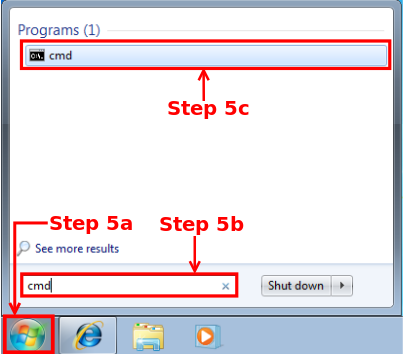
\includegraphics[width=0.4\textwidth]{dia9}
\end{center}
\vspace{-0.5cm}
\caption{Accessing the command line from the Start Menu (steps 5a-5c.)}
\label{fig:dia9}
\end{figure}
\item A Command Line window should appear. Type ``python'' and press Enter.
Python should begin running, as shown in Figure \ref{fig:dia10}.
\begin{figure}[h]
\begin{center}
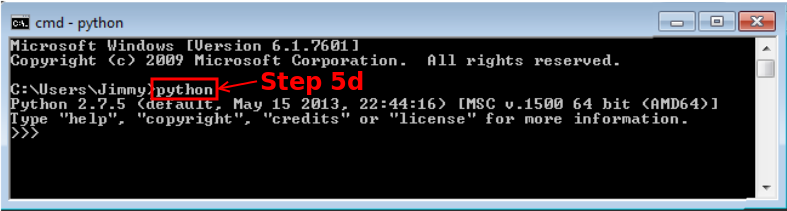
\includegraphics[width=0.8\textwidth]{dia10}
\end{center}
\vspace{-0.5cm}
\caption{The Windows Command Line running the Python Interpreter (step 5d.)}
\label{fig:dia10}
\end{figure}
\end{enumerate}
{\Large {\bf Conclusion}}
\myhrule
You may now begin entering Python commands. To use Python in the future, repeat
step 5.
\end{document}
